%%%%%%%% ICML 2018 EXAMPLE LATEX SUBMISSION FILE %%%%%%%%%%%%%%%%%

\documentclass{article}

% Recommended, but optional, packages for figures and better typesetting:
\usepackage{microtype}
\usepackage{graphicx}
\usepackage{subfigure}
\usepackage{booktabs} % for professional tables

% hyperref makes hyperlinks in the resulting PDF.
% If your build breaks (sometimes temporarily if a hyperlink spans a page)
% please comment out the following usepackage line and replace
% \usepackage{icml2018} with \usepackage[nohyperref]{icml2018} above.
\usepackage{hyperref}

% Attempt to make hyperref and algorithmic work together better:
\newcommand{\theHalgorithm}{\arabic{algorithm}}

% Use the following line for the initial blind version submitted for review:
% \usepackage{icml2018}

% If accepted, instead use the following line for the camera-ready submission:
\usepackage[accepted]{icml2018}

% The \icmltitle you define below is probably too long as a header.
% Therefore, a short form for the running title is supplied here:
\icmltitlerunning{Project Proposal for CS234 (Winter 2019)}

\begin{document}

\twocolumn[
\icmltitle{Project Proposal for CS234 (Winter 2019) \\
			Reinforcement Learning under Incomplete Information: \\
			Learning to Play Stratego}

% in order of appearance and this is the preferred way.
\icmlsetsymbol{equal}{*}

\begin{icmlauthorlist}
\icmlauthor{Li Quan Khoo}{stanford,scpd}
\end{icmlauthorlist}

\icmlaffiliation{stanford}{Computer Science Department}
\icmlaffiliation{scpd}{Stanford Center for Professional Development}

\icmlcorrespondingauthor{Li Quan Khoo}{lqkhoo@stanford.edu, li.khoo.11@ucl.ac.uk}

% You may provide any keywords that you
% find helpful for describing your paper; these are used to populate
% the "keywords" metadata in the PDF but will not be shown in the document
\icmlkeywords{Machine Learning, ICML}

\vskip 0.3in
]

% this must go after the closing bracket ] following \twocolumn[ ...

% This command actually creates the footnote in the first column
% listing the affiliations and the copyright notice.
% The command takes one argument, which is text to display at the start of the footnote.
% The \icmlEqualContribution command is standard text for equal contribution.
% Remove it (just {}) if you do not need this facility.

\printAffiliationsAndNotice{}  % leave blank if no need to mention equal contribution
% \printAffiliationsAndNotice{\icmlEqualContribution} % otherwise use the standard text.

\graphicspath{{img/}} % set of paths to search for images

\section{Description of Stratego}

Stratego is an incomplete information 2-player turn-based game, on a square grid board. Depending on the variant played, each player starts with a number of pieces, numbering from 40 (Classic), 20 (Lightning), 10 (Duel), to 8 (Blitz) in total.

\begin{figure}[H]
	\centering
	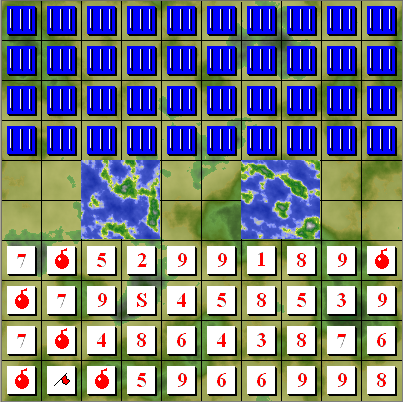
\includegraphics[width=.75\linewidth]{Stratego}
	\caption{Classic Stratego board. In this image, higher number means lower rank.}
\end{figure}

The objective is to capture the opponent's Flag. Each piece has a rank, and generally, pieces of higher rank can capture any lower-ranked piece. Capturing a piece of the same rank removes both from the board. All pieces can move one square in the 4 cardinal directions. Exceptions are: Scouts can move any number of squares, Bombs and Flags cannot move, and the Spy can capture the highest-ranked piece. For full rules, refer to \cite{ISFrules}.

When capturing, an arbiter decides the outcome, and sometimes only partial information about the opponent's piece is revealed. For example, if a rank 3 piece attacks another piece but is itself removed, the other piece could either be a Bomb, or any piece of at least rank 4.

Similar games to Stratego include Luxiangqi, Jungle (the blind-play variant), and Banqi (sometimes called Chinese Blind Chess). They share the same concept of having varied initial states, and unknown starting rank for the opponent's pieces.

\section{Why reinforcement learning?}
Reinforcement learning is used in many areas, but unless we have perfect simulation, usually we can find a better way to do it \cite{rlblogpost}. For example, I have considered setting this project topic in locomotion using MuJoCo, but many real world problems are better solved using a combination of kinematics and optimization, to make use of domain knowledge in physics \cite{tassa2012}, \cite{kuindersma2016}.

Abstract games are the notable exception, as we have perfect simulation by definition, and they are not bound by the physical world.

\section{Complexity}
Classic stratego has an upper-bound of $10^{115}$ states (chess: $10^{45}$, go: $10^{172}$). However, its game-tree complexity is $10^{535}$ nodes (chess: $10^{123}$, go: $10^{360}$), due to long play-length \cite{arts10}.

Stratego is also a two-phase game. The first phase involves setting up the initial piece positions, and the second phase involves moving the pieces. In our project, to manage complexity, we will likely build up from versions with fewer pieces up to Lightning (20 per player).

\section{Prior work}
Stratego is not a well-studied game, since at best, it exists in the fringes of mainstream board games. I found a CS231N project \cite{smith2015} which attempted to solve Stratego using alpha-beta pruning and tree-search, called perfect information Monte-Carlo Sampling (PIMCS) \cite{long2010}. However, instead of maintaining a value function, the author fitted a CNN using 15k game states to determine the probability of winning, which is not updated by the agent's subsequent play. Given the size of Stratego's state space, I'm not sure if this is a good idea. \cite{arts10} also looked at tree search methods for Stratego in his thesis.

\section{Why is this interesting?}
Unlike other imperfect information games, such as poker, where some probability distribution over the opponents' hands could be inferred over the course of play based on the cards revealed, in Stratego, the game gradually reveals information about each piece throughout the game, but there is also a cost to each reveal. This makes it such that each interaction between pieces is like a bandit, which also modifies the values which all other pieces (bandits) returns, since once revealed, the probability distribution of ranks over each opponent piece changes.

In the cases where the opponent's pieces have been completely determined, Stratego degenerates to a perfect information game. It would be interesting to find a strategy that works when only some pieces have been completely determined. In contrast, it would be very difficult or impossible in blackjack to be able to determine that one of your opponent's cards is an ace, or that your opponent has a particular tile in mahjong.

In between the different Stratego variants, the fewer the pieces, the more random the outcome would be (as pieces are sacrificed to reveal information). However, the more pieces there are, the less information is revealed each time (as the probability distribution is over more pieces).

\section{Evaluation}
This was the most difficult part of the project to determine. There was a tournament hosted by a now-defunct organization called StrategoUSA for Stratego AIs. The last tournament was held in 2010, and the winner algorithm was called Probe, which was distributed as Windows binary, but it is no longer available from anywhere. The 2009 winner was called Master of the Flag II (available at http://www.jayoogee.com/masteroftheflag/game.html)

Due to the lack of scripting interfaces and source code, it is likely that we will have to manually input the agent's moves into these interfaces, to evaluate against a baseline. However, these baselines only play the Classic version. The only other way to measure relative improvement over time is to make sure later versions of the agent win more games than it loses (on average) when played against all earlier versions of the agent, whose policies are not as refined yet.

\section{Scope}
\begin{enumerate}
\item First, we have to implement a rule-conformant version of Stratego, including rules such as the two-squares rule, instead of redefining an easier draw condition, if we want to play against Master of the Flag II. We also need a way to input moves and starting states when the agent is not playing against itself.
\item We need a visualization scheme to understand what is going on.
\item We need to implement and train the neural net, which consists of a convolutional input network, and at least a value network.
\item We need a reward function.
\end{enumerate}

% In the unusual situation where you want a paper to appear in the
% cesces without citing it in the main text, use \nocite
\nocite{langley00}

\bibliography{proposal}
\bibliographystyle{icml2018}



\end{document}

